\documentclass[11pt,a4paper]{article}
\usepackage[T1]{fontenc}
\usepackage[utf8]{inputenc}
\usepackage[ngerman]{babel}
\usepackage{geometry}
\usepackage{graphicx}
\usepackage{tabularx}
\usepackage{booktabs}
\usepackage{longtable}
\usepackage{array}
\usepackage{hyperref}
\usepackage{xcolor}
\usepackage{enumitem}
\usepackage{float}
\usepackage{titlesec}
\usepackage{caption}

\geometry{margin=2.3cm}
\hypersetup{
  colorlinks=true,
  linkcolor=black,
  urlcolor=blue,
  pdftitle={usability - Refinement},
  pdfauthor={[Vorname Nachname eintragen]}
}

\setlength{\parindent}{0pt}
\setlength{\parskip}{0.7em}
\captionsetup{font=small, labelfont=bf}
\titleformat{\section}{\large\bfseries}{\thesection}{0.7em}{}
\titleformat{\subsection}{\normalsize\bfseries}{\thesubsection}{0.7em}{}

\newcommand{\studentname}{[Vorname Nachname eintragen]}
\newcommand{\moduletitle}{usability - Refinement}

\begin{document}

\begin{titlepage}
\centering
\vspace*{2.5cm}
{\Huge\bfseries \moduletitle \par}
\vspace{1.8cm}
{\Large Dokumentation einer analytischen Evaluation und des anschließenden Refinements \par}
\vspace{2.2cm}

\begin{tabular}{ll}
\textbf{Name:} & \studentname \\
\textbf{Projekt:} & Flight Delay Explorer \\
\textbf{Abgabeformat:} & PDF-Dokumentation zur Evaluation \\
\textbf{Kontext:} & Big-Data-Dashboard / Streamlit-Anwendung \\
\textbf{Evaluationsart:} & analytische Evaluation (Expert Review / Heuristic Evaluation) \\
\end{tabular}

\vfill

{\large
Aufgabenstellung: Evaluieren Sie Ihr Programm entweder unter Verwendung einer analytischen Evaluationsmethode oder unter Anwendung einer empirischen Evaluationsmethode mit mindestens fünf Proband:innen. Dokumentieren Sie die Evaluation mit allgemeiner Beschreibung der Methode, tatsächlichem Evaluationsverlauf, Auswertung und Fazit.
\par}

\vspace{1.2cm}
{\large \today \par}
\end{titlepage}

\tableofcontents
\newpage

\section{Einleitung}
Im vorliegenden Projekt wurde die Anwendung \textit{Flight Delay Explorer} auf Usability-Schwächen untersucht und anschließend gezielt verbessert. Die Anwendung ist ein datenintensives Dashboard zur Analyse von Flugverspätungen, Annullierungen, Routen, Flughäfen und Airlines. Gerade bei einem solchen System ist gute Usability entscheidend, weil Nutzer:innen schnell zwischen Überblick, Filterung und Detailansicht wechseln müssen. Wenn wichtige Hinweise schlecht lesbar sind, wenn Visualisierungen nur über Farben funktionieren oder wenn Karten nur per Maus verständlich sind, sinkt die Effektivität der Anwendung sofort.

Für diese Aufgabe wurde bewusst eine \textbf{analytische Evaluationsmethode} gewählt. Der Grund dafür ist, dass das Projekt bereits über eine funktionierende Anwendung verfügt und die wichtigsten Risiken zunächst effizient auf Basis etablierter Richtlinien identifiziert werden sollten. Statt einer Proband:innen-Studie stand hier eine strukturierte heuristische Überprüfung im Vordergrund. Das passt besonders gut, weil sich zentrale Probleme wie Kontrast, Farbkodierung, Tastaturbedienbarkeit oder Informationsdichte bereits ohne Labor- oder Feldstudie belastbar prüfen lassen.

\section{Datenbasis der Anwendung}
\subsection{Verwendete Datensätze}
Die Anwendung basiert auf mehreren lokalen Datensätzen, die gemeinsam ein analytisches Bild des US-amerikanischen Flugverkehrs im ersten Quartal 2024 liefern:

\begin{itemize}[leftmargin=1.2cm]
\item drei BTS-Flugdatenarchive für Januar, Februar und März 2024,
\item \texttt{airports.csv} als Flughafen-Lookup,
\item \texttt{runways.csv} zur Anreicherung mit Start- und Landebahndaten,
\item \texttt{airport-frequencies.csv} zur zusätzlichen Flughafenbeschreibung,
\item \texttt{countries.csv} und \texttt{regions.csv} für Länder- und Regionsnamen.
\end{itemize}

Die Flugdaten bilden die zentrale Faktentabelle. Die Flughafentabelle wird zweimal an die Flüge gejoint, einmal für den Origin-Flughafen und einmal für den Destination-Flughafen. Runways und Frequenzen werden vor dem Join aggregiert, damit keine Zeilenvervielfachung entsteht.

\subsection{Welche Informationen in den Daten enthalten sind}
Die drei BTS-Monatsdateien enthalten pro Flug jeweils fachlich zentrale Merkmale wie Flugdatum, Airline-Code, Origin- und Destination-Airport, geplante und tatsächliche Abflug- bzw. Ankunftszeiten, Abflug- und Ankunftsverspätungen, Flugdistanz, Informationen zu Annullierung und Umleitung sowie die Aufteilung der Verspätung auf einzelne Ursachen. Dazu gehören insbesondere \textit{Carrier Delay}, \textit{Weather Delay}, \textit{NAS Delay}, \textit{Security Delay} und \textit{Late Aircraft Delay}.

Für die Anwendung wurden diese Rohdaten zusätzlich bereinigt und erweitert. Beispiele für abgeleitete Merkmale sind:

\begin{itemize}[leftmargin=1.2cm]
\item \texttt{route} und \texttt{route\_id} für die Analyse konkreter Verbindungen,
\item \texttt{flight\_month\_name} und \texttt{flight\_weekday\_name} für zeitliche Vergleiche,
\item \texttt{departure\_hour}, \texttt{arrival\_hour} und \texttt{time\_of\_day\_group} für Tageszeitmuster,
\item Delay-Flags und On-Time-Klassifikationen für KPI-Karten,
\item \texttt{distance\_group} für Kurz-, Mittel- und Langstrecken,
\item \texttt{main\_delay\_cause} als dominierende Verspätungsursache pro Flug.
\end{itemize}

Gerade diese Anreicherung ist für die Visualisierung wichtig: Erst dadurch lassen sich Seiten wie \textit{Time Analysis}, \textit{Delay Causes}, \textit{Route Analysis} oder der Vergleichsmodus fachlich sinnvoll und gleichzeitig gut filterbar aufbauen.

\subsection{Umfang und Relevanz für die Evaluation}
Die Datenbasis ist für die Usability-Evaluation wichtig, weil sie die Komplexität der Benutzeroberfläche direkt bestimmt. Große Datenmengen bedeuten viele Filter, viele Vergleichsmöglichkeiten und potenziell überladene Visualisierungen.

\begin{table}[H]
\centering
\caption{Zentrale Datenkennzahlen der Anwendung}
\begin{tabularx}{\textwidth}{lXr}
\toprule
\textbf{Kategorie} & \textbf{Beschreibung} & \textbf{Wert} \\
\midrule
Zeilen in der kombinierten Flugtabelle & Januar bis März 2024 & 1.658.259 \\
Quellarchive & monatliche ZIP-Dateien & 3 \\
Zeitraum & minimale bis maximale Flugdatumsausprägung & 01.01.2024 bis 31.03.2024 \\
Airlines & unterschiedliche Fluggesellschaften in der gefilterten Faktentabelle & 15 \\
Origin-Flughäfen & eindeutige Abflughäfen & 334 \\
Destination-Flughäfen & eindeutige Zielflughäfen & 334 \\
Join-Qualität & Flüge ohne Origin-Match / Destination-Match & 0 / 0 \\
\bottomrule
\end{tabularx}
\end{table}

Beispielhaft zeigen die Daten auch die analytische Breite der Anwendung: Die Airline mit dem größten Verkehrsanteil in der Gesamtauswahl ist \texttt{WN}, der verkehrsreichste Origin-Flughafen ist \texttt{ATL}, und besonders häufige Routen sind unter anderem \texttt{OGG -> HNL} und \texttt{LAX -> SFO}. Diese Datenfülle macht die Anwendung fachlich wertvoll, erhöht aber gleichzeitig die Anforderungen an Orientierung, Lesbarkeit und Informationsreduktion.

\subsection{Bedeutung der Lookup-Daten für Karte und Detailansichten}
Die Lookup-Dateien sind nicht nur technische Hilfstabellen, sondern bestimmen direkt den Mehrwert des Dashboards. Über \texttt{airports.csv} erhält die Anwendung reale Flughafencodes, Namen, Städte, Länder sowie geographische Koordinaten. Diese Koordinaten werden in der Kartenansicht verwendet, damit Flughäfen als echte Punkte auf der USA-Karte erscheinen und Routen als Linien bzw. Bögen zwischen realen Start- und Zielorten gezeichnet werden können.

Die Dateien \texttt{runways.csv} und \texttt{airport-frequencies.csv} ergänzen zusätzliche Strukturinformationen zu Flughäfen, werden aber bewusst zuerst pro \texttt{airport\_ident} aggregiert. Dadurch bleibt die Flugdatenbasis stabil und wird nicht künstlich vervielfacht. Für die Evaluation war das relevant, weil nur so belastbar geprüft werden konnte, ob Kennzahlen, Kartenpunkte und Ranking-Tabellen fachlich korrekt bleiben.

\section{Allgemeine Beschreibung der Evaluationsmethode}
\subsection{Sinn und Zweck}
Die gewählte Methode ist eine \textbf{analytische Evaluation in Form eines Expert Reviews}. Dabei wird die Anwendung systematisch gegen Gestaltungs- und Usability-Richtlinien geprüft, ohne dass dafür zunächst Proband:innen benötigt werden. Der Sinn dieser Methode liegt in der schnellen und strukturierten Identifikation typischer Schwachstellen:

\begin{itemize}[leftmargin=1.2cm]
\item Lesbarkeitsprobleme,
\item inkonsistente oder missverständliche Visualisierungen,
\item fehlende Alternativen für Tastatur- oder Screenreader-Nutzung,
\item kognitive Überlastung durch zu dichte Layouts,
\item Brüche im Prinzip ``Overview first, zoom and filter, details on demand''.
\end{itemize}

Ziel war nicht nur, Probleme zu benennen, sondern daraus einen konkreten Refinement-Plan abzuleiten und diesen anschließend schrittweise umzusetzen.

\subsection{Bewertungsgrundlagen}
Die Prüfung orientierte sich an drei Quellenarten:

\begin{enumerate}[leftmargin=1.2cm]
\item dem lokalen Kurs-/Gestaltungsdokument mit Visualisierungs- und Usability-Regeln,
\item WCAG-2.2-Kriterien, insbesondere zu Kontrast, Farbe, Alternativtexten und Tastaturbedienung,
\item einer seitenweisen Inspektion der real laufenden Anwendung.
\end{enumerate}

\subsection{Typischer Ablauf einer analytischen Evaluation}
Der allgemeine Ablauf lässt sich in vier Schritte gliedern:

\begin{enumerate}[leftmargin=1.2cm]
\item \textbf{Prüfkriterien festlegen}: Welche Richtlinien und Heuristiken sind für den Anwendungstyp relevant?
\item \textbf{Systematische Inspektion}: Alle Hauptseiten, Filter, Diagramme, Tabellen und Interaktionspfade durchgehen.
\item \textbf{Befunde dokumentieren und priorisieren}: Probleme nach Schweregrad und Auswirkung sortieren.
\item \textbf{Verbesserungen ableiten und re-evaluieren}: Maßnahmenplan formulieren, umsetzen und erneut überprüfen.
\end{enumerate}

\section{Tatsächlicher Evaluationsverlauf}
\subsection{Durchführung des Befund-Scans}
Der eigentliche Usability-Scan wurde manuell durchgeführt, also ohne Agentenunterstützung bei der Suche nach Schwächen. Bewertet wurden die Hauptseiten \textit{Overview}, \textit{Time Analysis}, \textit{Airline Analysis}, \textit{Airport Analysis}, \textit{Route Analysis}, \textit{Delay Causes}, \textit{Cancellation and Diversion}, \textit{Map View}, \textit{Flight Table Explorer}, \textit{Comparison Mode} und \textit{Data Quality}. Zusätzlich wurden die globale Filterleiste, die Detailansichten und die Karteninteraktion betrachtet.

Die Inspektion erfolgte mit folgenden Leitfragen:

\begin{itemize}[leftmargin=1.2cm]
\item Sind Texte, Hinweise und Beschriftungen gut lesbar?
\item Funktionieren Visualisierungen auch dann, wenn Farben allein nicht ausreichen?
\item Gibt es textliche Alternativen oder tabellarische Fallbacks?
\item Sind Interaktionen auch ohne Maus verständlich und erreichbar?
\item Unterstützt das Layout eher den Überblick oder überlastet es auf kleinen Bildschirmen?
\end{itemize}

\subsection{Dokumentierte Hauptbefunde}
Der analytische Scan führte zu zwei \textbf{High}- und vier \textbf{Medium}-Befunden:

\begin{table}[H]
\centering
\caption{Zusammenfassung der identifizierten Usability-Lücken}
\begin{tabularx}{\textwidth}{>{\bfseries}l l X}
\toprule
Priorität & Kategorie & Kurzbeschreibung \\
\midrule
High & Lesbarkeit & Sekundärtexte lagen unter dem geforderten WCAG-AA-Kontrast und waren für erklärende Hinweise zu schwach. \\
High & Verständlichkeit & Mehrere zentrale Visualisierungen transportierten Bedeutung primär über Farbe. \\
Medium & Zugänglichkeit & Diagramme hatten oft keine direkte Textalternative oder tabellarische Zusammenfassung. \\
Medium & Bedienbarkeit & Die Karte war stark mauszentriert und bot keine gleichwertige Tastatur-Interaktion. \\
Medium & Responsive Nutzung & Mehrere Seiten waren visuell dicht und auf kleineren Ansichten unnötig schwer zu scannen. \\
Medium & Robustheit & Ein Teil der Primärdarstellung beruhte auf Custom-HTML statt auf nativen Komponenten. \\
\bottomrule
\end{tabularx}
\end{table}

Diese Befunde wurden in einem internen Reviewprotokoll festgehalten. Anschließend wurde daraus ein vierphasiger Maßnahmenplan abgeleitet.

\section{Auswertung der Evaluation}
\subsection{Interpretation der Befunde}
Die Befunde zeigen, dass die Anwendung bereits fachlich stark und visuell attraktiv war, aber an typischen Stellen einer datenreichen Dashboard-Anwendung nachgeschärft werden musste. Besonders auffällig war das Spannungsfeld zwischen ``schön'' und ``zugänglich'': Die Oberfläche wirkte modern und hochwertig, doch gerade dabei wurden einige klassische Usability-Risiken sichtbar.

Die kritischsten Probleme betrafen nicht die Datenlogik, sondern die Vermittlung der Information:

\begin{itemize}[leftmargin=1.2cm]
\item Wenn Untertexte zu schwach kontrastieren, helfen sie ihren eigentlichen Nutzern nicht mehr.
\item Wenn Farbe die einzige Codierung ist, entstehen Barrieren für Farbsehschwächen und allgemein für schnelle Interpretation.
\item Wenn Karten nur über Hover/Pointer funktionieren, werden Tastatur- oder Screenreader-Pfade faktisch abgeschnitten.
\item Wenn zu viele Informationen gleichzeitig nebeneinander stehen, leidet der Erstzugang zur Anwendung.
\end{itemize}

\subsection{Abgeleiteter Refinement-Plan}
Aus der Auswertung wurde folgender Maßnahmenplan abgeleitet:

\begin{enumerate}[leftmargin=1.2cm]
\item \textbf{Phase 1 -- Accessibility-Blocker}: Kontrastkorrekturen und Ende der farb-exklusiven Bedeutungsvermittlung.
\item \textbf{Phase 2 -- Selbsterklärende Visualisierung}: Chart-Summaries, Tabellen-Fallbacks und zugänglichere Kartenbedienung.
\item \textbf{Phase 3 -- Mobile und Erstnutzung}: Leichtere Seitenstrukturen, weniger dichte Mehrspalten-Layouts, bessere Detailführung.
\item \textbf{Phase 4 -- Robustheit}: Mehr Nutzung nativer Streamlit-Komponenten statt rein dekorativer HTML-Blöcke für zentrale Informationsbereiche.
\end{enumerate}

\section{Umgesetztes Refinement Schritt für Schritt}
Der Plan wurde anschließend nicht nur formuliert, sondern tatsächlich umgesetzt.

\subsection{Phase 1: Kritische Accessibility-Fixes}
Zuerst wurde der Kontrast der sekundären Texte erhöht. Dazu wurde der bisherige ``muted''-Farbton abgedunkelt und kleine KPI-Labels optisch verstärkt. Parallel dazu wurden Visualisierungen so angepasst, dass Bedeutung nicht mehr nur über Farbe transportiert wird. Beispiele dafür sind:

\begin{itemize}[leftmargin=1.2cm]
\item zusätzliche Linienstile in Mehrlinien-Charts,
\item Pattern Shapes in gestapelten Balkendiagrammen,
\item textliche Severity-Bands auf der Karte,
\item stärkere Umrissbreiten bei unterschiedlich kritischen Kartenpunkten.
\end{itemize}

\subsection{Phase 2: Verständlichkeit und Alternativen}
Im zweiten Schritt erhielten die wichtigsten Visualisierungen kurze ``How to read''-Erläuterungen. Zusätzlich wurde unter jedem relevanten Chart ein aufklappbarer Tabellen-Fallback ergänzt. Damit existiert nun neben der Visualisierung immer auch eine strukturierte, zugängliche Darstellung der gleichen Information.

Die Karte wurde außerdem um eine tastaturfreundliche Auswahl ergänzt: Flughäfen und Routen lassen sich nun nicht nur per Hover oder Klick in der Karte, sondern auch per Selectbox auswählen. Die Detailinformationen erscheinen anschließend in einer strukturierten Tabelle.

\subsection{Phase 3: Mobile und First-Use-Refinement}
Im dritten Schritt wurden besonders dichte Seiten reduziert. Statt unnötig vieler paralleler Spalten wurden mehrere Bereiche auf eine vertikale Leselogik umgestellt. Auf kleineren Ansichten stapeln sich Hero-Bereich, KPI-Kacheln und erklärende Elemente nun kontrollierter. Zusätzlich wurden einzelne Detailbereiche in Tabs überführt, um die Erstorientierung zu verbessern.

\subsection{Phase 4: Robustheit und Konsistenz}
Abschließend wurden zentrale Informationsblöcke stärker auf native Streamlit-Komponenten verlagert, insbesondere bei Hinweisen, Detailtabellen und erläuternden Panels. Das visuelle Branding blieb erhalten, aber die robusteren und besser zugänglichen Standardkomponenten wurden dort bevorzugt, wo echte Inhalte und Interaktionen im Vordergrund stehen.

\section{Screenshots des finalen Zustands}
Die folgenden Abbildungen zeigen den nach dem Refinement erreichten Stand der Anwendung.

\begin{figure}[H]
\centering
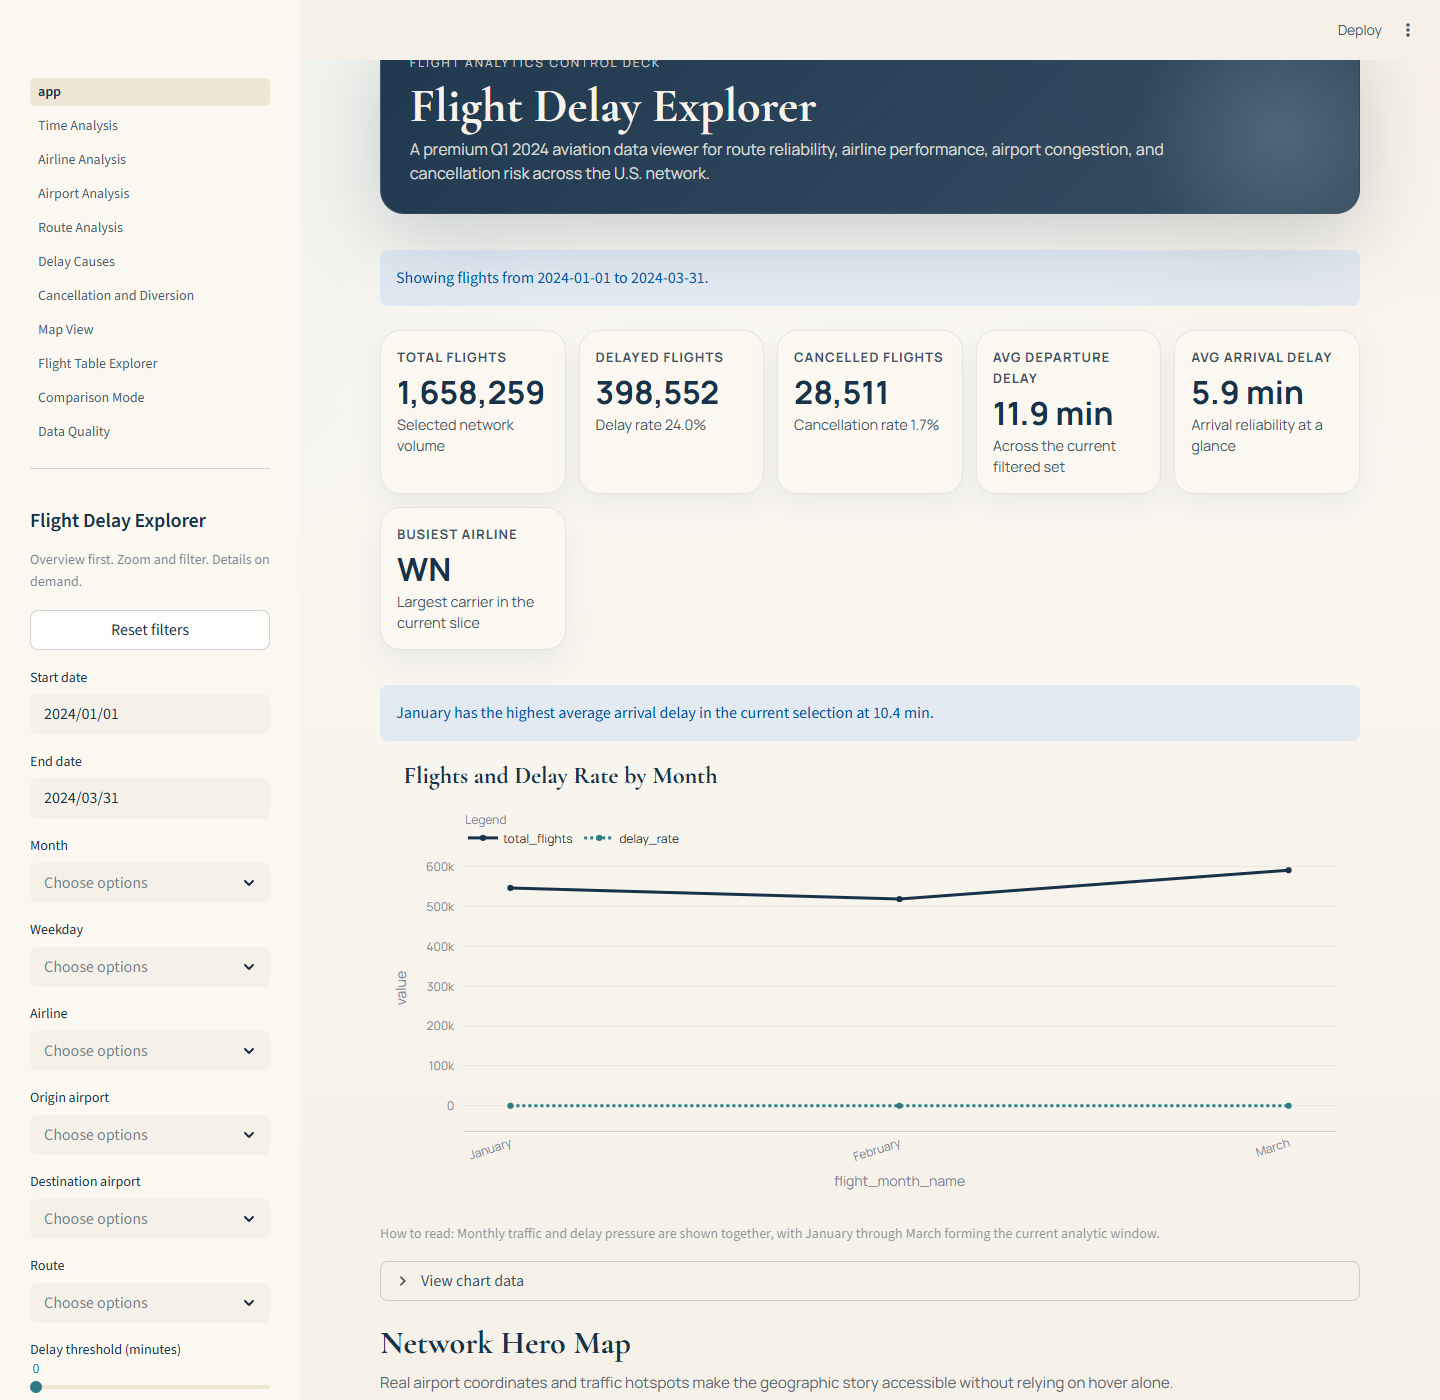
\includegraphics[width=\textwidth]{screenshots/01_overview.png}
\caption{Overview-Seite nach dem Refinement: KPI-Überblick, klarere Lesbarkeit, ``How to read''-Hinweise und zugänglicher Einstieg in Diagramm und Karte.}
\end{figure}

\begin{figure}[H]
\centering
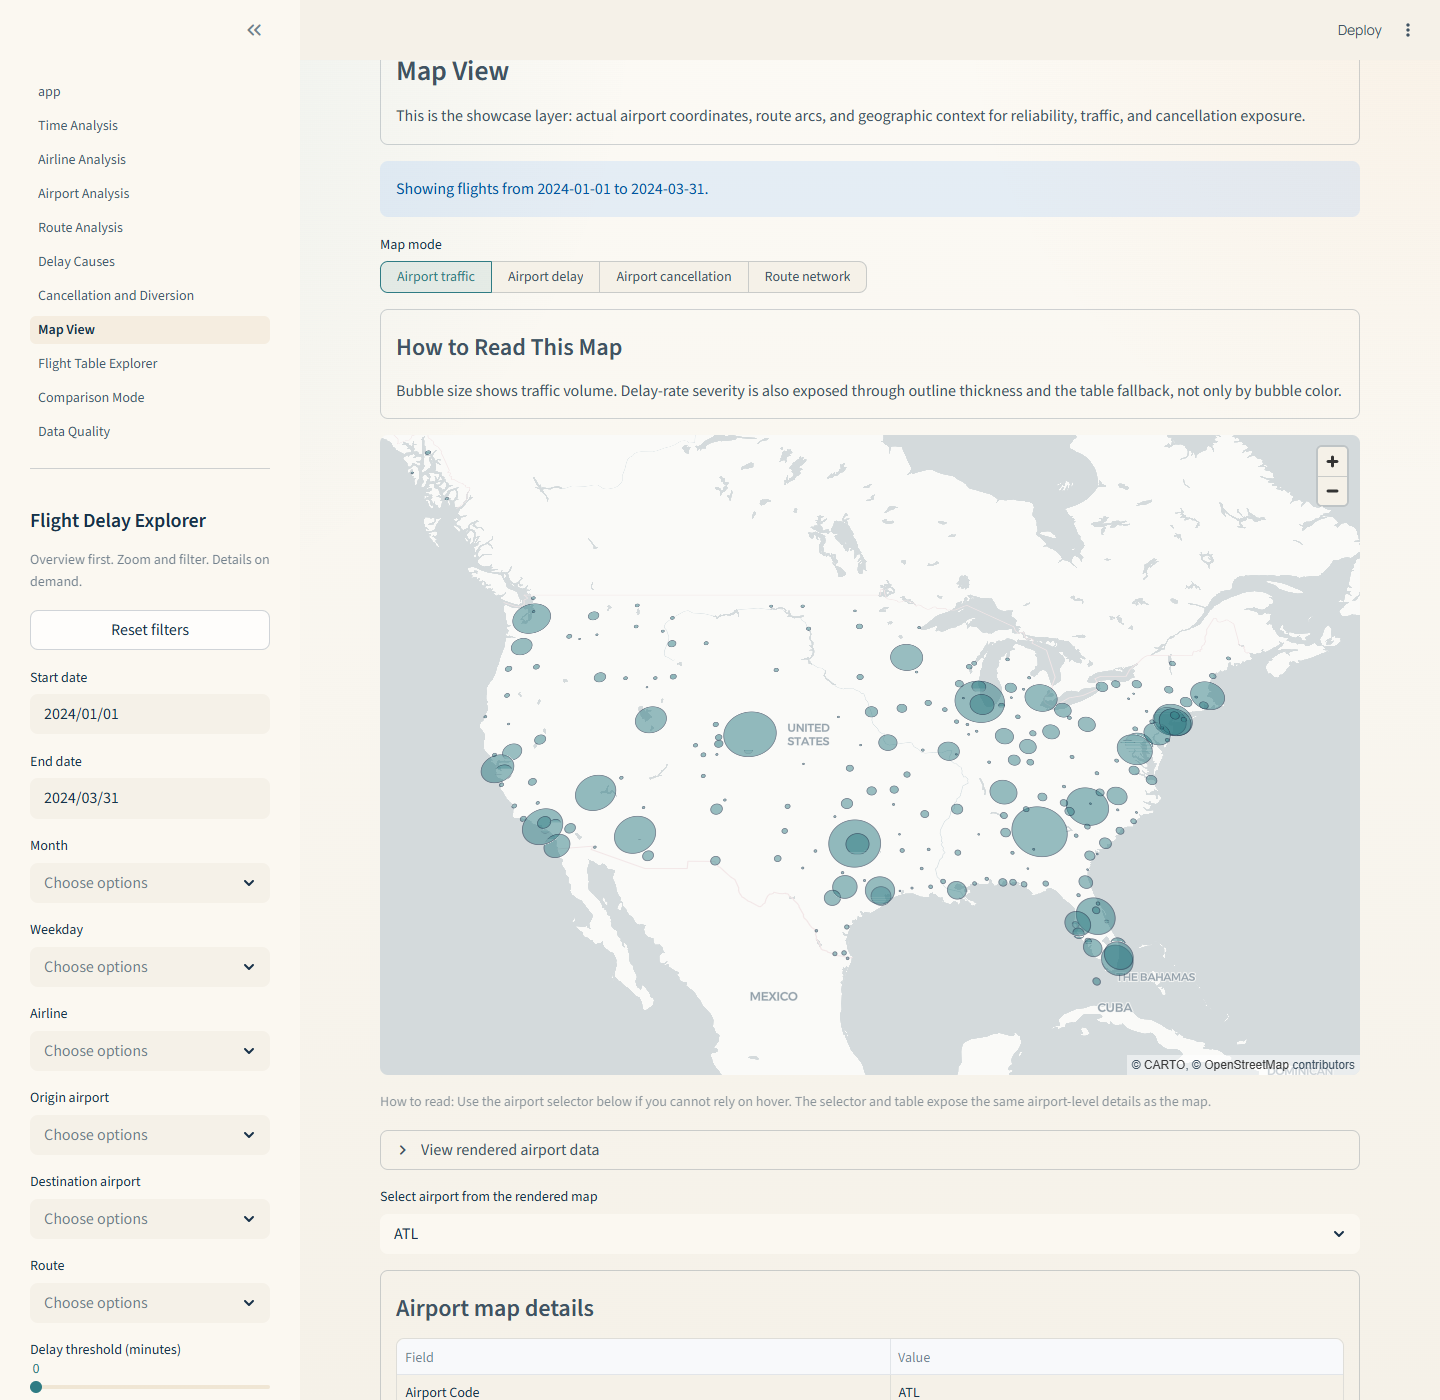
\includegraphics[width=\textwidth]{screenshots/02_map.png}
\caption{Map View nach dem Refinement: textliche Lesehilfe, tastaturfreundliche Flughafenauswahl und strukturierte Kartendetails als Alternative zu Hover-Interaktion.}
\end{figure}

\begin{figure}[H]
\centering
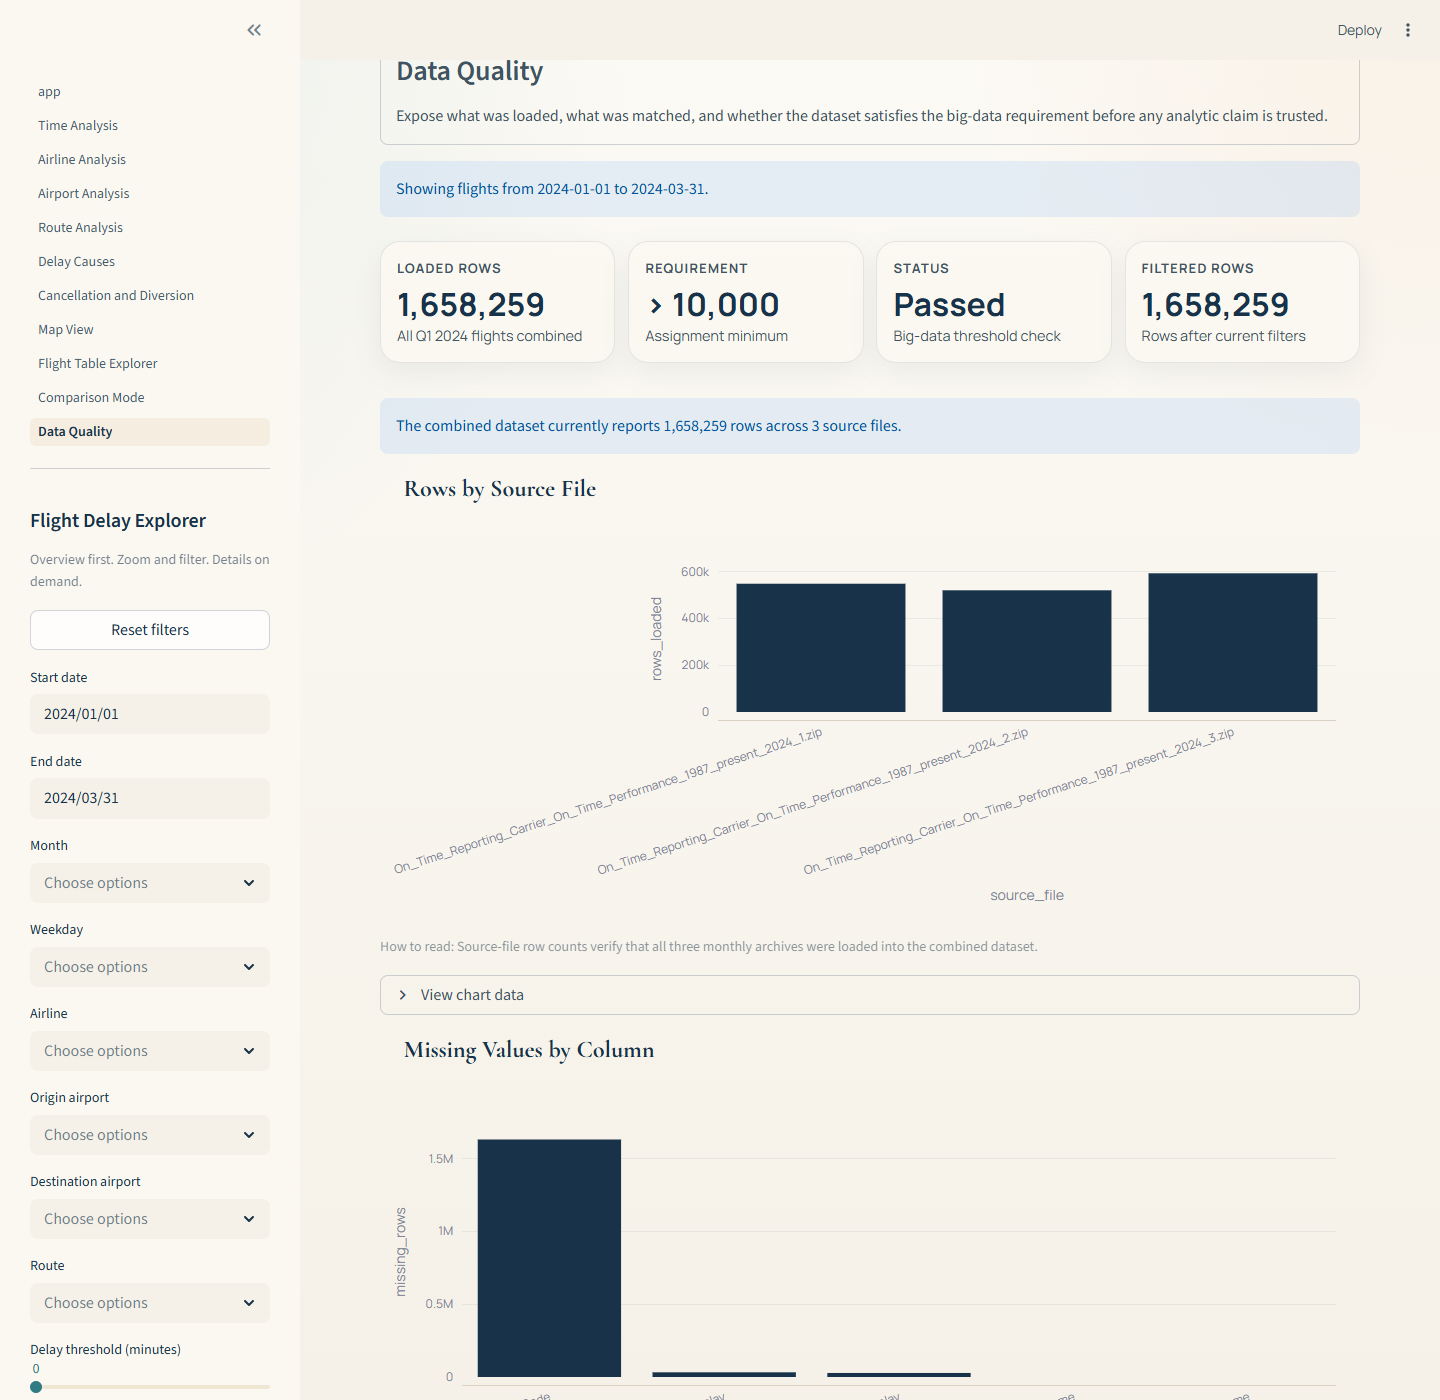
\includegraphics[width=\textwidth]{screenshots/03_data_quality.png}
\caption{Data-Quality-Seite: nachvollziehbare Qualitätsübersicht mit Datenumfang, Quellarchiven, Missingness und verständlichen Detailtabellen.}
\end{figure}

\section{Prompt-Logbuch (rekonstruiert und hypothetisch)}
Wichtig ist: Der \textbf{Usability-Scan selbst} wurde als manuelle analytische Evaluation durchgeführt, also \textbf{ohne Agentenprompt zur Identifikation der Lücken}. Das folgende Prompt-Logbuch dokumentiert nur hypothetische bzw. rekonstruierte Prompts für die \textbf{Planung} und \textbf{Umsetzung} der Verbesserungen.

\begin{longtable}{p{0.08\textwidth} p{0.22\textwidth} p{0.62\textwidth}}
\toprule
\textbf{Nr.} & \textbf{Zweck} & \textbf{Rekonstruierter Prompt} \\
\midrule
\endfirsthead
\toprule
\textbf{Nr.} & \textbf{Zweck} & \textbf{Rekonstruierter Prompt} \\
\midrule
\endhead
1 & Maßnahmenplan erstellen & \texttt{Erstelle auf Basis dieser dokumentierten Usability-Befunde einen konkreten, priorisierten Refinement-Plan für unsere Streamlit-Anwendung. Ordne die Maßnahmen nach Impact und Aufwand und formuliere klare Phasen mit Akzeptanzkriterien.} \\
2 & Accessibility-Blocker beheben & \texttt{Implementiere Phase 1 des Refinement-Plans: bessere Textkontraste, keine farb-exklusive Bedeutungsvermittlung mehr, redundante Encodings in Charts und Karten. Ändere nur das Nötige, aber validiere die App danach technisch.} \\
3 & Chart-Summaries und Tabellen-Fallbacks & \texttt{Setze Phase 2 um: Füge zu allen wichtigen Visualisierungen kurze verständliche Erklärungen und einen zugänglichen Daten-Fallback hinzu. Sorge außerdem für eine tastaturfreundliche Alternative zur Karteninteraktion.} \\
4 & Mobile/First-Use-Polish & \texttt{Reduziere auf den wichtigsten Seiten unnötig dichte Zwei-Spalten-Layouts, verbessere die Scanbarkeit auf kleineren Screens und ersetze rohe Detail-Dumps durch strukturierte Detailansichten.} \\
5 & Finaler Feinschliff & \texttt{Führe einen Low-Effort-High-Impact-Polish-Pass durch: klarere Lesehinweise an Charts, leichtere Reihenfolge auf kleinen Screens, bessere Legenden und kurze Validierung der laufenden App.} \\
\bottomrule
\end{longtable}

\section{Fazit}
Die analytische Evaluation hat gezeigt, dass das Projekt bereits fachlich stark war, die Benutzerfreundlichkeit aber an mehreren zentralen Stellen gezielt verbessert werden musste. Besonders wichtig war dabei die Erkenntnis, dass gute Visualisierung nicht nur ``schön'', sondern auch zugänglich, robust und interpretierbar sein muss.

Die größten Verbesserungen wurden durch relativ klar abgrenzbare Maßnahmen erreicht: besserer Kontrast, keine Bedeutungsvermittlung nur über Farbe, textliche Hilfen für Visualisierungen, Tabellen-Fallbacks, tastaturfreundliche Karten-Alternativen und leichtere Seitenlayouts. Dadurch wurde die Anwendung nicht nur barriereärmer, sondern auch für Erstnutzer:innen verständlicher.

Insgesamt lässt sich festhalten, dass die analytische Evaluationsmethode für dieses Projekt sehr sinnvoll war. Sie erlaubte eine schnelle, systematische und quellenbasierte Identifikation von Usability-Lücken. Durch den anschließenden Refinement-Prozess wurden diese Lücken nicht nur beschrieben, sondern konkret geschlossen. Für einen möglichen nächsten Schritt wäre eine ergänzende empirische Evaluation mit fünf Proband:innen sinnvoll, um die nun optimierte Anwendung zusätzlich im realen Nutzungskontext zu überprüfen.

\newpage
\section*{Quellenverzeichnis}
\addcontentsline{toc}{section}{Quellenverzeichnis}

\begin{itemize}[leftmargin=1.2cm]
\item \textbf{Lokale Projektquelle:} \texttt{Flight Delay Explorer App Instructions.pdf}
\item \textbf{Lokale Projektquelle:} \texttt{dashboard\_design\_guidelines\_ GPT Generiert.docx}
\item \textbf{Lokale Projektquelle:} Interner analytischer Reviewbericht, Datei \texttt{pasted-text.txt} (lokale Arbeitsunterlage).
\item \textbf{Datengrundlage:} \texttt{On\_Time\_Reporting\_Carrier\_On\_Time\_Performance\_1987\_present\_2024\_1.zip}, \texttt{\_2.zip}, \texttt{\_3.zip}, \texttt{airports.csv}, \texttt{runways.csv}, \texttt{airport-frequencies.csv}, \texttt{countries.csv}, \texttt{regions.csv}
\item \textbf{WCAG 2.2 -- Use of Color:} \url{https://www.w3.org/WAI/WCAG22/Understanding/use-of-color.html}
\item \textbf{WCAG 2.2 -- Non-text Content:} \url{https://www.w3.org/WAI/WCAG22/Understanding/non-text-content.html}
\item \textbf{WCAG 2.2 -- Contrast (Minimum):} \url{https://www.w3.org/WAI/WCAG22/Understanding/contrast-minimum.html}
\item \textbf{WCAG 2.2 -- Keyboard:} \url{https://www.w3.org/WAI/WCAG22/Understanding/keyboard.html}
\item \textbf{Eigene Abbildungen:} Screenshots der lokal laufenden Anwendung, erzeugt am 28.06.2026 aus dem finalen Stand des Flight Delay Explorer.
\end{itemize}

\end{document}
